\chapter{Úvod}
\chapter{Přehled teorie}
\label{prehled}

V teto kapitole jsou popsaný teoretické základy Petřino sítí. Taky tato kapitola se soustředí na popis několika podtříd Petriho sítě, zejména na „vysokoúrovňové Petriho sítě“ a „Značkované Petriho Sítě“ a  včetně přehledu míst, kdě se tento modelovací prostředek používá, a hra významnou roli.

Dalším účelem této kapitoly je seznámení čtenáře s matematickými popisy Petriho síti a grafy Petriho sítí, které jsou nezbytné pro porozumění principu prací simulátoru.

Do obsahu patří popis protokolu MQTT \ref{subsec:mqtt-proto}, na kterém je založena externí komunikace simulátoru \ref{subsec:mqtt_impl}.

Taky se tady zmíní o simulační teorii, zaměřené na simulaci Petriho síti v reálném čase. Vyjasní se pojem distribuovaných systému \ref{subsec:distr_system}, HWIL \ref{subsec:hwil} a jejích vztah z Petriho sítěmi.

\subsection{Petriho sítě}
V současné době se Petriho sítě často používají jako modelovací prostředek pro modelovaní chovaní systému, za účelem pochopení jeho slabších stránek, ještě než se system nasadí do provozu. Vyplňuje, tím pádem, díru mezi slovním popisem, návrhem, takovými modelovacími prostředky jako \href{https://en.wikipedia.org/wiki/Unified_Modeling_Language}{UML} a skutečnou implementací nějakého projektu. Použití Petriho síti pro účel modelování je velice vhodné, jen velmi málo modelovacích prostředku dokáže popsat ne jenom system jako celek, ale i zjistit slabší stránky jeho implementace, ještě před implementační fází. Stejně tak platí i pro testovací fází -- některé chyby se dá objevit jenom po implementací, když to Petriho sítě částečně řeší tento problém ještě ve fází navrchu.

\paragraph{Definice}

Petriho síť ($PN$) se sestavuje ze čtyřce prvku, $PN = \left(P, T, I, O\right)$ kde:
  \begin{itemize}
    \item $P = \left\{p_1, p_2, \cdots , p_n\right\}$ je konečná množina míst, $n >= 0$; \\
    \item $T = \left\{t_1, t_2, \cdots , t_m\right\}$ je konečná množina přechodů, $m >= 0$; \\
    \item $I = T \rightarrow P^\infty$ je vstupní funkce, propojující přechody s množinou vstupních míst; \\
    \item $O = P \rightarrow T^\infty$ je výstupní funkce, propojující výstupní místa s množinou přechodů; \\
  \end{itemize}
P $\vee$ T = $\varnothing$, P $\wedge$ T != $\varnothing$.

\section{Typy Petriho sítě}

\subsection{Značkované Petriho sítě}
Značkované petriho seti (ZPS) zavadí takový pojem jako značka nebo \uv{token}. Značka je základní prvek v ZPS, umožnující její vykonávaní. Vykonávaní se provádí provedením přechodu, během kterého se vymaže odpovídající počet značek ze množiny vstupních míst, a do výstupních míst se potřebný počet značek vloží. Tato operace se muže vykonávat dokud nezbude žádný povoleny přechod. Na tento myšlence je založena simulace provádění Petriho sítě.

Přechod v PS je povolen, dokud každé ze vstupních míst propojených s daným přechodem obsahuje alespoň jednu značku.

Pri vykonávaní sítě Petri, vznikají dvě posloupnosti - posloupnost značek a posloupnost přechodu, které byly provedeny. Teto dve posloupnosti zcela popisuji vykonání Petriho sítě.
%[Petri net theory and model... par:2.4 p 18-19]

Kazda ze šipek v Petriho sítí ma váhu. Váha reprezentuje číslo tokenů, které se musí nacházet ve vstupním místě pro to, aby přechod byl proveditelný. Pří provedení váha určuje kolík tokenů se vyjme ze vstupního místa, nebo kolík se jích vloží do místa výstupního.

\paragraph{Definice}

Značkovaná Petriho sit je šestice $PN = \left(P, T, I, O, W, M_0\right)$
\begin{itemize}
  \item $P = \left\{p_1, p_2, \cdots , p_n\right\}$ je konečná množina míst, $n >= 0$; \\
  \item $T = \left\{t_1, t_2, \cdots , t_m\right\}$ je konečná množina přechodů, $m >= 0$; \\
  \item $I = T \rightarrow P^\infty$ je vstupní funkce, propojující přechody s množinou vstupních míst; \\
  \item $O = P \rightarrow T^\infty$ je výstupní funkce, propojující výstupní místa s množinou přechodů; \\
  \item $W = F \rightarrow \left\{1, 2, 3, \cdots \right\}$ je váhová funkce; \\
  \item $M_0$ je multimnožina počátečních značek;
\end{itemize}
P $\vee$ T = $\varnothing$, P $\wedge$ T != $\varnothing$.

Díky možnosti vykonávat Petriho sit, vzniká příležitost vytvořit simulační nastroj, který je založen na zmíněných teoretických základech. Podrobný popis simulace viz \ref{sec:implementation}.

\subsection{Časované petriho sítě}
Podtřída Časovaných petriho seti [Timed Petri Net] rozšiřuje pojem Značkovaných Petriho sítí o jednu důležitou zásadu -- přechod muže byt označen časovou funkcí. Aby se takový přechod provedl, ten čas musí uplynout, až potom se vyjmou tokeny ze vstupních míst, a vloží se do výstupních. Časová funkce nemusí být konstantní, ale v rámci této prací se použilo jenom konstantní čekaní na přechod, jelikož chovaní simulátoru musí být deterministické. Více o implementačních detailech viz. \ref{subsec:timed_pl}.

\subsection{Vysokoúrovňové Petriho sítě}
\label{sec:hlpn}
Vysokoúrovňové petriho sítě (High Level Petri Nets) jsou dalším rozšířením Petriho sítí, které umožňují jednodušší modelovaní takových procesů, pro které jsou důležité výpočty a matematické výrazy. Celkově, je tento druh Petriho sítě pohodlnější pro modelovaní toku řízení kódu nějakého programu, a ve své podstatě připomíná grafické programování.

\paragraph{Definice}

High Level Petri Net (HLPN) je struktura $HLPN = \left( P; T; D; T_{ype}; P_{re}; P_{ost}; M_0\right) $ kde \cite[p.11--12]{pnstd54}:

\begin{itemize}
  \item $P$ je konečná množina míst. \\
  \item $T$ je konečná množina přechodu, pro kterou platí $\left(P \cup T = \varnothing\right)$. \\
  \item $D$ je konečná neprázdná množina domén, kde kazdy element domény se jmenuje typ. \\
  \item $T_{ype}$ : $P \cap T \rightarrow D$ je funkce pro přidaní typu do míst a určeni typu přechodu.
  \item $P_{re}$, $P_{ost}$ : $TRANS$ $\rightarrow$ $\mu PLACE$ jsou pre a post kondici pro které platí: \\
  \begin{center}
    \item $TRANS$ = $\left\{\left(t, m\right) | t \in T, m \in T_{ype} \left( t \right)\right\}$ \\
    \item $PLACE$ = $\left\{\left(p, g\right) | p \in P, g \in T_{ype} \left( p \right)\right\}$ \\
  \end{center}
  \item $M_0$ je $\mu PLACE$ je multimnožina počátečních značek.
\end{itemize}

\subsection{Pravidlo pro provedeni přechodu}
Pokud je dane ze konečná multimnožina $T_\mu$ je zapnuta pro značku $M$, tedy přechod v $HLPN$ muže byt proveden pro značku $M'$ následujícím způsobem \cite[p.~12]{pnstd54}:
\begin{center}
  $M' = M - Pre(T_\mu) + Post(T_\mu)$
\end{center}


\subsection{$HLPN$ Graf}
Graf $HLPN$ ma následující vlastnosti:
\begin{itemize}
  \item $Graf\:site$ je sestaveny s dvou prvku - $mist$ a $tansici$, které jsou propojeny mezi sebou šipkami ($arks$).
  \item $Typy\:mist$ Každé místo musí mít přiraženy jeden typ. Množina typu nesmí byt prázdna.
  \item $Znackovani\:mist$: je kolekce prvku, které musejí odpovídat typu místa, ve kterém se nacházejí. Prvky se jmenuji $tokeny$ a můžou se opakovat.
  \item $Sipkove\:annotaci$: kazda šipka je anotovaná výrazem se sestavujícím z konstant, proměnách ($x, y$) nebo funkci($f(x)$). Kazda proměna je typovaná, a výrazy se provádějí přiražením hodnot ke každé ze proměnách. Vyhodnoceni výrazu produkuje kolekci prvku převzatých ze vstupního místa. Kolekce se muže opakovat.
  \item $Podminky\:pro\:přechod$: jsou booleově výrazy ve tvaru $x < y$, které jsou zapsané v anotaci tranzite.
  \item $Deklaraci$: Vytvářejí definici typu míst, funkci a proměnách.
\end{itemize}

\subsection{Aplikace Petriho sítí}

\subsection{Značkovaná Petriho sít}
Rozsah míst kdě se dá aplikovat Petriho sítě je velmi široký. Jako modelovací prostředek můžou sloužit například pro reprezentací vzorů interakce a vznikájicich konfliktů mezí člověkem a autopilotem letadla, jak je popsané v následujícím \href{https://www-tandfonline-com.ezproxy.lib.vutbr.cz/doi/full/10.1080/00140139.2013.877597}{článku}.

Příkladem použiti značkované petriho sítí muže taky sloužit implementace \uv{Dining philosophers problem} \cite[p.65--67]{PNandMoS}, což je problém poprvé představeny profesorem Dijkstrou v roce 1965.
Je to obecné známy problém paralelismu, který názorné zobrazuje dva případy chyb vznikajících pri paralelním vypočtu - vyhladověni a uváznutí \cite{dining_philosophers}.

\subsection{Vysokoúrovňová Petriho sit}

V našem případě vysokoúrovňová Petriho síť modeluje a následně simuluje chování systému topení.

\subsection{Distribuovaný system}
\label{subsec:distr_system}

\paragraph{Definice}

Definice distribuovaného systému zni:
Distribuovaný system je kolekce na sobe nezávislých počítačů, který konečný uživatel vnímá jako celek.
% http://barbie.uta.edu/~jli/Resources/MapReduce&Hadoop/Distributed%20Systems%20Principles%20and%20Paradigms.pdf

Distribuované systémy musejí používat decentralizované algoritmy, které požaduji následující:
\begin{enumerate}
  \item Žádný prvek nesmí vědět informaci o celkovém stavu systému.
  \item Prvek uvazuje jenom na základe jeho stavu.
  \item Chyba v žádném z prvku ne ovlivni chovaní algoritmu.
  \item Neprovádí se synchronizace podle globálních hodin.
\end{enumerate}

Z definice taky vyplývá, ze distribuovaný system se obecně sestavuje s více se opakujících prvku, které funguji nezávisle na sobe a nemají přistup ke sdílené paměti, neboli kazdy prvek ma svob vlastni. Sdíleni stavu ve případe distribuovaného systému se provádí pomoci zasílaní zprav.

Tento koncept je velice použitelný pro modelovaní. Prvky budou reprezentovaný Petriho sítěmi, provázané komunikačními kanály. Jelikož kazda petriho sit je prvek nezávislý na vnějších podmínkách, ale jen na současném stavu mist a přechodu a taky jejich kombinaci, tak se da to prohlásit decentralizovaným algoritmem. Petriho sit si můžeme představit jako nezávislý blok, kdežto pro komunikaci mezi těmito bloky se da použit protokol \href{http://docs.oasis-open.org/mqtt/mqtt/v3.1.1/csprd02/mqtt-v3.1.1-csprd02.html}{MQTT}, který díky svým vlastnostem dokaze obsloužit neomezené množství klientu najednou. Případ implementace tepelného řízeni \ref{sec:tepelne-rizeni} názorné ukazuje použiti dane myšlenky na praktice.

\subsection{Simulace}
\subsection{Diskrétní simulace}
Diskrétní simulace je založena ve svém základu na algoritmu známém pod názvem \uv{NextEvent}. Tento algoritmus se řídí nasledujícím pseudokodem:
\begin{algorithm}
  \caption{Diskrétní simulace}\label{euclid}
  \begin{algorithmic}[1]
  \State $\text{nainicializuj simulaci, cas a planovac udalosti}$
  \While {dokud je naplánovaná událost}
  \State $\text{vyjmi prvni udalost ze seznamu}$
  \If {\texttt{cas\_udalosti >= T\_END}}
    \Return
  \EndIf
  \State $\text{nastav cas na cas udalosti}$
  \State $\text{proved popis chovani udalosti}$
  \EndWhile
  \end{algorithmic}
  \end{algorithm}
\subsection{Simulace v reálném čase}
Simulace v reálném čase se lisí of diskrétní simulace v jedné vlastnosti. Běh takové simulace musí byt synchronizován s relacím časem. 

Simulace v reálném čase upravena pro účely tohoto projektu je založena na výše zmíněném algoritmu \uv{Next Event} s jedinou změnou, která přidává čekaní na synchronizaci simulačního času s reálným, nebo na příchod nové události. Algoritmus v tom případe vypadá následujícím způsobem:

\begin{algorithm}
\caption{Real-time simulace}\label{euclid}
\begin{algorithmic}[1]
\State $\text{nainicializuj simulaci, cas a planovac udalosti}$
\While {dokud je naplánovaná událost}
\State $\text{podivej se na cas dalsi udalosti}$
\If {\texttt{cas\_udalosti >= T\_END}}
\Return
\EndIf
\State $\text{pockej na cas udalosti nebo na prichod nove udalosti}$
\If {\texttt{nova\_událost}}:
    \State \texttt{Continue}
\EndIf
\State proveď popis chovaní události
\EndWhile
\end{algorithmic}
\end{algorithm}

Tento algoritmus nachází svoje použiti ve mnoha simulačních případech. Běžný příklad použiti -- počítačové hry, kde uživatele zaujme herní prostředí, které simuluje reální svět, včetně časové roviny. Simulace v reálném čase se taky používá, kdy obyčejné diskrétní simulace nestačí a cas není zanedbatelný. Uživatel muže chtít sledovat system v průběhu simulace, za účelem zjištěni anomálii v chovaní jeho prvku nebo zvýšeni kvality systému prev jeho nasazením do provozu. Takový přistup se používá ve případě simulace \hyperref[subsec:hwil]{\uv{Hardware-in-the-loop}}.

\subsection{Hardware-in-the-loop(HWIL)}
\label{subsec:hwil}

Hardware-in-the-loop nebo HIL je technika používaná pro vývoj a testovaní řídicích častí komplexních systémů. Díky níž se fyzické častí systému nahrazují jejích simulaci a umožňují plynulé testovaní ještě před nasazením do provozu \cite{hil}.

\subsection{MQTT protokol}
\label{subsec:mqtt-proto}

\href{http://mqtt.org/}{MQTT} je protokol určeny pro komunikaci ve případech nízké propustnosti síti nebo její vysoké nespolehlivosti. V současné době svoje využiti nachází v \href{https://en.wikipedia.org/wiki/Internet_of_things}{IoT}. MQTT zavadí takové pojmy jako \hyperref[par:client]{klient}, \hyperref[par:broker]{broker}, \hyperref[par:message]{zpráva} a \hyperref[par:topic]{téma}. Dále nasledují popisy důležitých častí protokolu MQTT z daného zdroje \cite{mqtt}.

\paragraph{MQTT Klient}
\label{par:client}

Klient je tenká aplikace, schopna navázaní spojeni s brokerem. K jeho vlastnostem patří podpora odebíraní zpráv pomoci filtrovaní na základě parametru, zvanému \hyperref[par:topic]{\uv{topic}}. MQTT klient muže byt použit pro zařízeni, jejichž výkon je bod srazu, díky lehkosti MQTT protokolu.

\paragraph{MQTT Broker}
\label{par:broker}

Broker je server, obsluhující klienty, navazuje spojeni s klientem a provádí přeposíláni zprav typu \texttt{PUBLISH}, které odebírají téma, nacházející ve hlavičce zprávy. Každý klient se přípojí k brokeru tak, že otevře sezení, během kterého může se serverem komunikovat. Pro tén účel klient musí předem vědět IP adresu brokeru, která pro něj bude přístupní.

\paragraph{Téma}
\label{par:topic}

Kazda zprava posílaná klientem se nepředává primo dalšímu klientovi, ale obsluhuje se brokerem. Zprava musí mit specifikované téma, podle které broker určí, kterým klientům tu zprávu musí přeposlat. Takové téma je obvykle unikátní textový řetězec, který bude následně odebírat jeden či více klientů.

Zvláštní význam má, ve případě MQTT tématu, znak \uv{\#} (U+0023). Téma se obecně skládá z 1 až několika řetězců, které jsou oddělené znakem \uv{/} (U+002F). Pokud takové téma končí značkou \uv{\#}, tak je výsledek totožný z \uv{wildcard} znakem \uv{*} (U+002A) z \href{https://en.wikipedia.org/wiki/Regular_expression}{regulárních výrazů}.

\begin{tabbing}
 Příklad: \= \\
 \> \texttt{net1/\#} -- přijímá zprávy na téma \texttt{net1}, \texttt{net1/port1}, \texttt{net1/port1/log} atd.\\
 \> \texttt{net2/portX} -- přijímá zprávy jenom na téma \texttt{net2/portX}. \\
\end{tabbing}

Příklady aplikace tohoto pojmu můžete vidět na příkladě \ref{code:remote-in-out}, nebo jiných aplikací \todo{}.

\paragraph{Zpráva}
\label{par:message}

Zprávy musejí mit specifikovaný obsah, a parametr QoS. Obsah zprávy je tělo samotné zprávy, které dostane klient a na základě ní se bude jednat dál. Obsah se posílá v bytech, a pro případ zprávy typu \texttt{PUBLISH}, může být prázdný.

QoS muže byt 3 typu:
\begin{itemize}
  \item $QoS_0$ -- Nanejvýš jedno dodaní.
  \item $QoS_1$ -- Alespoň jedno dodaní.
  \item $QoS_2$ -- Přesně jedno dodaní.
\end{itemize}

Podle hodnoty tohoto parametru se určí, jak důkladně se bude obsluhovat zpráva.

\paragraph{Tok nastavení}

Pro navázaní spojeni s brokerem po nastaveni sítového připojeni s adresou brokeru, klient musí nejdříve poslat zprávu \texttt{CONNECT}, obsahující vlastní identifikátor. Na tu zprávu server musí odpovědět zprávou typu \texttt{CONNACK} potvrzující navázaní spojeni a nulovým návratovým kódem. Potom klient je volen poslat zprávy typu \texttt{SUBSCRIBE} s tématem na které chce dostávat zprávy a hodnotou \texttt{QoS}. Server odpovídá zprávou \texttt{SUBACK}, návratová hodnota je ve případě úspěchu je menší nebo rovná se hodnotě \texttt{QoS}. Potom uz zprava typu \texttt{PUBLISH} z určitým obsahem od klienta který provedl všechny minule kroky bude zpracovaná brokerem.

\begin{figure}[hbt]
  \centering
  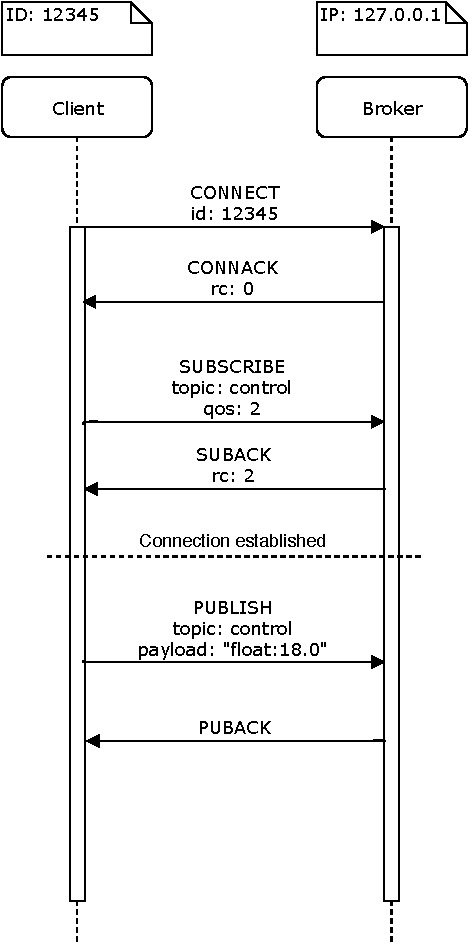
\includegraphics[width=0.5\textwidth]{obrazky-figures/MQTT-flow.pdf}
  \caption{Ukázka komunikace Klientu a Brokeru.}
  \label{mqtt-flow}
\end{figure}

\chapter{Implementace}
\label{sec:implementation}

\subsection{Knihovna $SNAKES$}

\href{https://www.ibisc.univ-evry.fr/~fpommereau/SNAKES/}{\texttt{SNAKES}} -- je knihovna v jazyce Python která nabízí všechno potřebné pro definici a spouštěni několika variant Petriho sítí. Cílem knihovny \texttt{SNAKES} je nabídnout badatelům možnost rychle namodelovat novy nápad. Zvláštní vlastnosti knihovny \texttt{SNAKES} je možnost vytvářet Barevné Petriho site s použitím výrazů v jazyce Python pro anotaci přechodu ci vstupních nebo výstupních šipek. \cite{snakes}

Zvláštní vlastnosti \texttt{SNAKES} je možnost implementace vlastních rozšířeni pro jednotlivé častí Petriho sítí, nebo přidaní nových vlastnosti pro modelovaní jiných podtypu Petriho sítí. Tato vlastnost byla zvlášť použita v této prací pro přidaní rozšířeni \ref{sec:plug-impl}, podporující vytvářeni Petriho sítí určených pro modelovaní distribuovaných systému.

\subsection{Implementace MQTT}
\label{subsec:mqtt_impl}
Pro implementací mqtt klientu v simulátoru byla použitá knihovna \href{https://pypi.org/project/paho-mqtt/}{\texttt{paho-mqtt}}. Tato knihovna obsahuje všechno potřebné pro nastavení komunikačních kanálů mezí porty vzdálených Petriho sítí. Na základě použití této knihovny konečný uživatel může nastavit zvolené místo v Petriho sítí jako vstupní nebo výstupní port. viz \ref{code:remote-in-out}. Jejích vzhled je následující:
\begin{figure}[hbt]
  \centering
  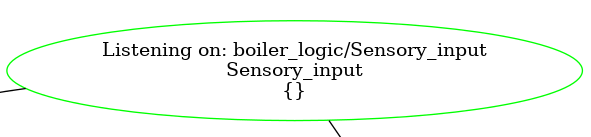
\includegraphics[width=0.5\textwidth]{obrazky-figures/port-in.png}
  \caption{Příklad vstupního portu}
  \label{port-in}
\end{figure}

\begin{figure}[hbt]
  \centering
  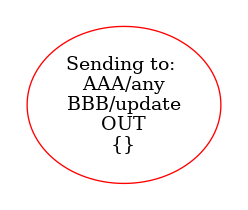
\includegraphics[width=0.5\textwidth]{obrazky-figures/port-out.png}
  \caption{Příklad výstupního portu}
  \label{port-out}
\end{figure}

Jak si můžete povšimnout, na rozdíl od ostatních míst sítě, vstupní a výstupní porty se označují barvou a dodatečným popisem. Pro vstupní port \ref{port-in} je to \texttt{Listening on: NET/TOPIC} a zelení barva, \texttt{Sending to: NET/TOPIC} pro výstupní \ref{port-out}. Ten, ve své řáde je označen červeně.

Je předem definované, že každá simulační instance odebírá zprávy z tématu \texttt{control}. Je to ekvivalent broadkastové adresy u IP.

Implementace zevnitř vypadá podobně reprezentací samotných portů. Sít, pří volaní metody \texttt{add\_remote\_input} nastaví týp místa na vstupní, pak pošle zprávu na téma \texttt{control} obsahující dvojicí [jméno sítě, jméno místa], a uloží zprávu do čekací fronty. Pak, když se k brokeru přípojí nějaká simulační instance s požadovanou dvojicí síť--místo, tak se to oznámí všem ostatním simulačním instancím. To se zase provede zasíláním zprávy na téma \texttt{control}. Hned po příjetí takové zprávy se port nastaví a bude vykonávat svou činnost.

\subsubsection{Směřování}
Na jeden vstupní port může být přípojeno 0 až několik výstupních portů, nebo jinými slovy vstupní port přijímá všechny zprávy na svoje téma.

\begin{figure}[htb]
  \centering
  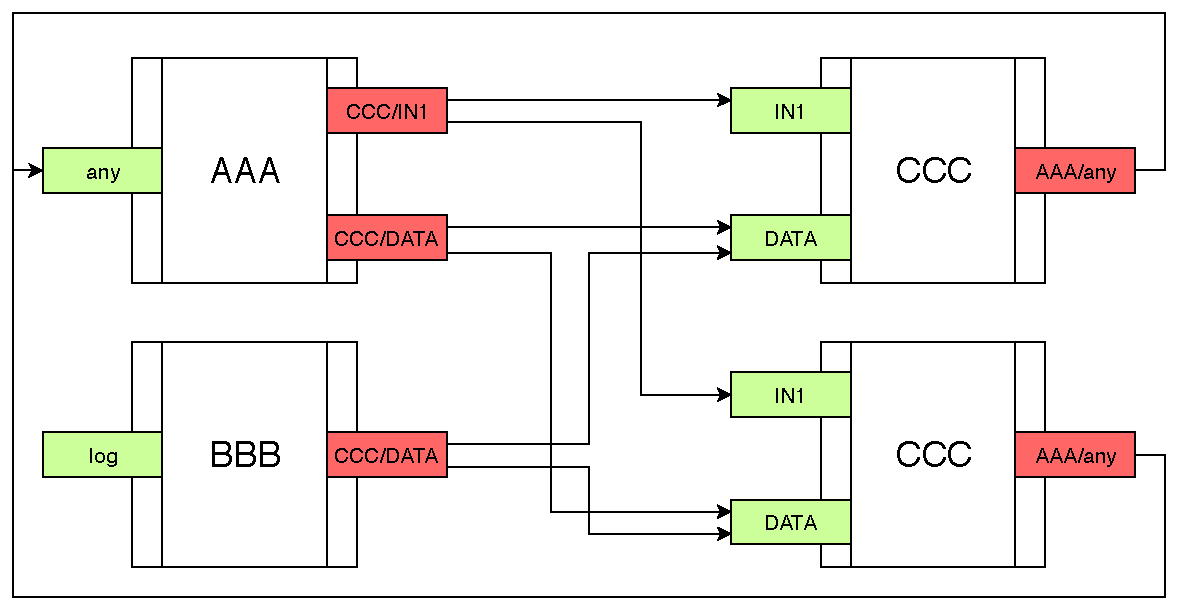
\includegraphics[width=0.7\textwidth]{obrazky-figures/Port-routing.pdf}
  \caption{Ukázka směřovaní zpráv.}
  \label{route-viz}
\end{figure}

Na danem výše obrázku \ref{route-viz} můžete vidět ukázku směřovaní zpráv mezí porty. \texttt{AAA}, \texttt{BBB} a \texttt{CCC} jsou identifikátory Petriho sítí v rámci jedeného brokeru. Ve případě že se dvojice síť--port se vyskytuje vícekrát, zprávy se přeposílají všem instancím. To si můžete všimnout na příkladu sítě \texttt{CCC}, která je na obrázku \ref{route-viz} dvakrát.

Na obrázku jsou 6 vstupních portů a 5 výstupních. Vstupní porty jsou označené zeleně, výstupní červeně. Jak je vidět na příklade dvojic \texttt{CCC/IN1} a \texttt{CCC/DATA}, dvojicí nemusí být unikátní. Počet přípojených výstupních portu k jedenému vstupnímu není nějak omezen. Je to dosažené použitím vlastností MQTT klientu popsané v \ref{par:topic}.

Na příkladě vstupního portu \texttt{log} můžete vidět že není povinné, aby ten port byl zapojený. Ve případě simulátoru takový port nebude přiřazen do skupiny vstupních portů, dokud se neobjeví nějaká aplikace nebo síť, požadující přijetí a odesílaní zpráv na téma, kterou ten port odebírá. Více se o takovém nastavení viz \todo{ADD}

\subsection{Vlastní protokol komunikace}
Proto aby simulator měl podporu přidání vzdálených portů, zmíněných v \ref{subsec:mqtt_impl} vznikla potřeba vymyslet vlastní protokol výměny informací. Ten protokol musí mít seznám zpráv pro takové simulační případy, kdy port musí předat nebo přijmout tokeny, nebo když se objeví instance Petriho síti v nějakém z už existujících či nově vytvořených simulačních uzlů. \todo{návod pro vytvoření takového}.

Následující tabulka \ref{tab:mqtt-msg-types} obsahuje přehled typů zpráv, a jejích formátu pro naplnění:

\begin{table}[H]
	\vskip6pt
	\caption{Tabulka typů zpráv}
    \vskip6pt
	\centering
	\begin{tabular}{llllr}
		\toprule
		Typ & Zkrátka & Formát \\
    \midrule
    Update & U & U\_ACTION, SRC\_SIM\_ID, NEW\_NET\_NAME \\
    Request & R & R\_ACTION, TARG\_NET/TARG\_PLACE, SRC\_NET/SRC\_PLACE \\
    Success & S & REQUEST\_COPY \\
    Failure & F & REQUEST\_COPY \\
		\bottomrule
	\end{tabular}
	\label{tab:mqtt-msg-types}
\end{table}

\paragraph{Update} Zprávy tohoto typu oznamují instancím simulátoru, jestli se v jejích okolí neobjevila nová Petriho síť, nebo naslouchající aplikace. Ve případě dodaní zprávy typu \uv{Update}, každá síť bude muset aktualizovat seznám svých aktivních portu, a ve případě že nějaký port čeká na nastavení, tak poslat požadavky na pro nově příchozího klienta. Poslední akcí je aktualizace tabulky známých sítí nově příchozího klienta, ve případě že klient není externí aplikace. Pro aplikaci je ten krok vynechán.
\todo{priklady}

\paragraph{Request} \label{par:request} Tento týp zpráv nastavuje vstupní a výstupní porty. Parametr \uv{\texttt{R\_ACTION}} může nabývat hodnoty \texttt{set\_input} pro nastavení cílového místa \uv{\texttt{TARG\_PLACE}} jako vstupní port pro síť \uv{\texttt{TARG\_NET}}. Parametr \uv{\texttt{SRC\_NET}} a \uv{\texttt{SRC\_PLACE}} není v tom případě potřeba, stačí uvést rozdělovač.

\begin{tabbing}
  Příklad: \= \\
  \>\texttt{R, set\_input, net1/port1, /}
\end{tabbing}

Pro nastavení výstupního portu stačí nastavit parametr \uv{\texttt{R\_ACTION}} na \texttt{set\_output} a dodat zdrojové místo a síť nastavením parametrů \uv{\texttt{SRC\_NET}} a \uv{\texttt{SRC\_PLACE}}.

\begin{tabbing}
  Příklad: \= \\
  \> \texttt{R, set\_output, net1/port1, net2/port2} \\
\end{tabbing}

\paragraph{Success} Táto zpráva se odesílá ve případě úspěšného zpracování nějakého požadavku z \ref{par:request}. Parametr \uv{\texttt{REQUEST\_COPY}} musí byt přesnou kopii příchozího požadavku.

\begin{tabbing}
  Příklad: \= \\
  \> \texttt{S, R, set\_output, net1/port1, net2/port2} \\
\end{tabbing}

Příjetí odesílající stranou potvrzovací zprávy Success, znamená že nastavení bylo úspěšné alespoň v jedněm případě, což má za následek nastavení místa s jménem \texttt{port1} sítě \texttt{net1} jako výstupní port do \texttt{net2/port2}.

\subsection{Implementace rozšíření}
\label{sec:plug-impl}
Tento pododdíl popisuje implementaci různých rozšíření pro knihovnu $SNAKES$, které znesnadňuji navrch Petriho sítí a její modelovaní. Každý z níže popsaných pluginů se da  použít v komu po jejích importu podle tohoto \href{https://www.ibisc.univ-evry.fr/~fpommereau/SNAKES/first-steps-with-snakes.html}{návodu}.

\subsection{Návod pro import rozšíření}
Vzhledem k odlišnému postupu pří přidání rozšíření do SNAKES, pro import simulačního nástroje a dalších rozšíření ze skupiny, uživatel musí dodrat správné pořadí pri importu knihoven. Konvence probíhá následujícím způsobem.

\begin{python}
  from snakes.nets import *   # Site, mista, prechody... (*\label{code:snakes-all}*) (*\label{code:plugin-setup}*)
  from simul import PNSim     # Simulacni knihovna (*\label{code:pnsim}*)
  snakes.plugins.load( (*\label{code:sim-plugins}*)
    ["gv", "timed_pl", "sim_pl", "prob_pl", "prior_pl"],
    "snakes.nets",
    "plugins") # Seznam rozsireni pro import
  from plugins import * # Redefinovane metody z rozsireni (*\label{code:pl-import}*)
\end{python}

\begin{enumerate}
  \item Přidaní knihovny snakes a její prvků \ref{code:snakes-all}.
  \item Import simulační knihovny, která poskytne základ pro rozšíření \ref{code:pnsim}.
  \item Přidaní pluginů podle požadovaných vlastností sítě \ref{code:sim-plugins}. Ze skupiny doporučených pluginů stojí za zmínku plugin \href{https://www.ibisc.univ-evry.fr/~fpommereau/SNAKES/API/plugins/gv.html}{\uv{gv}}. Více o jeho použití v rámci simulátoru viz.\ref{subsec:mereni-teploty}. Zbytek je popsán v dalších sekcích \ref{subsec:timed_pl}.
  \item Pro redefinici a přidání nových metod z rozšíření slouží řádek \ref{code:pl-import}. Od dané chvílí použití knihovny SNAKES je stejné jako v \href{https://www.ibisc.univ-evry.fr/~fpommereau/SNAKES/first-steps-with-snakes.html}{návodu} a taky \todo{Muj navod}.
\end{enumerate}

\subsubsection{Plugin \texttt{timed\_pl}}
\label{subsec:timed_pl}
Toto rozšířeni používá plánovač události pro spolehlivé plánovaní spouštěni tranzite do budoucna. Toto rozšířeni používá jednoduchou logiku pro provedeni přechodu - ve chvíli kdy přechod bude spustitelný, tak se zapne časovač a zkonzumuji odpovídající tokeny ze vstupních mist. Čekaní se neresetuje přidáním dalších tokenů do vstupních mist. Ve případe teto implementace přechod vezme nověpříchozí tokeny, které se objeví ve vstupních místech a tudíž zapnou přechod. Po ukončeni čekaní, tokeny budou přeneseny do výstupních mist, s následujícími úpravami, které můžou nastat podle definice HLPN \ref{sec:hlpn}.


\begin{python}
  # Vytvoreni prechodu s casovym spozdenim
  pr1=Transition("Timed-transition", timeout=30) (*\label{code:timed-example}*)
\end{python}

Pro vytváření takového přechodu stačí zadat parametr \texttt{timeout} do klauzule pro vytvoření přechodu - \texttt{Transition} jak je ukázano na řádku \ref{code:timed-example}. Hodnota \texttt{timeout} se uvádí v sekundách. Výsledný tvár nasledujícího přechodu je na obrázku \ref{timed-transition}. Ukázku použítí ve funkčním příkladě můžete vidět \hyperref[code:timed-temp-example]{dále}.

\begin{figure}[hbt]
  \centering
  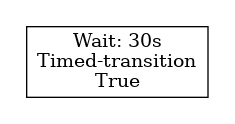
\includegraphics[width=0.3\textwidth]{obrazky-figures/timed-transition.png}
  \caption{Příklad časovaného přechodu}
  \label{timed-transition}
\end{figure}

\subsubsection{Plugin \texttt{prob\_pl}}
\label{subsec:prob_pl}
Toto rozsireni pridava moznost spojit nekolik tranzici do jedne skupiny, a tudiz rovnomerne rozdelit pravdepodobnost spousteni kazde z nich. Pro spojene přechody plati, ze museji mit stejnou sadu vstupnich mist. Pak se pri provedeni jedneho z nich se rozhodne na zaklade hodnoty jeho pravdepodobnosti jestli se tento přechod musi provest, nebo se provede nektery z jeho sousedu. Soucet pravdepodobnosti pro takovou skupinu přechodu musi byt vzdycky 1.

Takový přechod se definuje ve dvou krocích. Nejdříve se vytvaří prvek \texttt{Transition} s parametrem \texttt{prob}, jak je ukázáno na řádku \ref{code:prob-example}. Příklad použití v \hyperref[code:prob-ev-draw]{obecném} případě viz. řádek \ref{code:prob-temp-example}.
\begin{python}
  # Krok 1: Vytvoreni prechodu z parametrem prob
  pr1=Transition("Prob-trans-1", prob=0.6) (*\label{code:prob-example}*)
  pr2=Transition("Prob-trans-2", prob=0.4)
\end{python}

Dále stačí spojit pravdepodobnosti přechodu do jedné skupíny, pomoci klauzule \\ \texttt{add\_neighbour\_transition}. Viz. řádek \ref{code:prob-neghb-example} nebo řádek \ref{code:prob-temp-neghb-example} z kompletního \hyperref[code:prob-ev-draw]{příkladu}.
\begin{python}
  # Krok 2: Vytvoreni prechodu z parametrem prob
  pr1.add_neighbour_transition(pr2) (*\label{code:prob-neghb-example}*)
\end{python}

Tato sekvence vytvoří nasledující zobrazení - \ref{prob-transition}.

\begin{figure}[hbt]
  \centering
  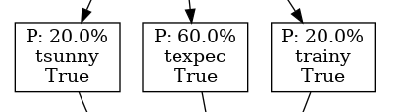
\includegraphics[width=0.6\textwidth]{obrazky-figures/prob-transition.png}
  \caption{Příklad pravděpodobnostního přechodu}
  \label{prob-transition}
\end{figure}

\subsubsection{Plugin \texttt{prior\_pl}}
\label{subsec:prior_pl}
Tento plugin je určeny pro přidaní prioritních pochodů do Petriho sítě. Podle nastavené priority se během simulace bude rozhodovat, který přechod se vyhodnotí a provede jako první. Priority můžou byt v rozsahu 0 -- 100, a radí se sestupné. Pro nastaveni priority element \texttt{Transition} má dodatečný a nepovinný parametr \texttt{prior} -- \ref{code:prior-transition-example}.
\begin{python}
  # Ukazka prioritniho prechodu
  tr=Transition('Enable boiler', prior=1) (*\label{code:prior-transition-example}*)
\end{python}

\begin{figure}[hbt]
  \centering
  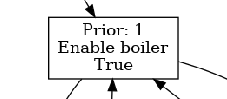
\includegraphics[width=0.3\textwidth]{obrazky-figures/prior-transition.png}
  \caption{Příklad prioritního přechodu s prioritou $1$}
  \label{prior-transition}
\end{figure}

\subsection{Plugin \texttt{sim\_pl}}
\label{sec:aplikace-mqtt}
Na implementací tohoto pluginu je založená práce ostatních pluginů ze skupiny \ref{sec:plug-impl}. Je ve své podstatě spojovacím prvkém mezi simulatorem, $MQTT$ klientem a sětí Petri. Obsahuje přetežovaní metod ze knihovny $SNAKES$ pro vykreslování prvků, které jsou rozšiřené pluginy. Taky přidavá zasadní metody pro nastavení Petriho sítě, umožnující použítí simulatoru a provadění spouštění sítě \ref{code:add_simulator}.
\begin{python}
  sim=PNSim() (*\label{code:sim-add}*)
  n=PetriNet("Sample net")
  n.add_simulator(sim) (*\label{code:add_simulator}*)
\end{python}

Stejně tak podporuje nastavení vzdalených portů pro předaní tokenů jiným sítím připojeným na stejnou adresu $MQTT$ brokeru \ref{code:remote_in}, \ref{code:remote_out}.

\begin{python}
  n.add_remote_input(it, "temp_gen/Measurement") (*\label{code:remote_in}*) (*\label{code:remote-in-out}*)
  n.add_remote_output(hen, "boiler_logic/Sensory_input") (*\label{code:remote_out}*)
\end{python}


\subsection{Planovac udalosti}
\label{subsec:event-planner}
Plánovač události je naimplementován jako prioritní fronta za využiti vestavěné knihovny \href{https://docs.python.org/3/library/heapq.html}{\texttt{heapq}} v Pythonu. Api naznačuje ze pro přidaní a vyberu prvku se používají metody \texttt{heappush} a \texttt{heappop}. Priorita v takové frontě se určuje číselnou hodnotou, která se vkládá do fronty. Tato hodnota muže byt prvním prvkem v seznamu elementu. Druhým parametrem pro určeni priority je poradí, ve kterém prvek byl vložen. Tato sada pravidel umožňuje vkládat záznamy, obsahující čas spuštěni jako první prvek, a podle toho se zařadí na přisluhující místo ve frontě. Metoda \texttt{heappop} vybere prvek ze seznamu s nejvyšší prioritou, což bude element s nejnižší hodnotou času.


\chapter{Aplikace}

\section{Tepelne rizeni}
\label{sec:tepelne-rizeni}
Pro demonstraci praci simulatoru bylo rozhodnuto namodelovat dystribovany system modelujici chovani topení, ktey nekteri z vas pravdepodobne pouzivaji u sebe doma. Takovy system se sestavuje z nekolika casti. Zakladnim prvkem je plynovy spotrebic, nebo karma. Ta ohriva vodu a uvadi ji do pohybu po potrubich. Pak kazdy z pokoju ma na starosti tepelené čidlo a rizeni, ktere udrzuje v pokoji nastavenou teplotu podle calendare. Kazdou hodinu se z tabulky teplot vezme aktualni teplota pro soucasnou hodiny a tento pokoj, pak rizeni rozhodne jestli ma zapnout topení nebo ne. Pokud zadny z pokoju v soucasne dobe nema zapnute topení, tak karma se musi vypnout za ucelem setreni plynu. Toto rizeni provadi vestaveny system, nebo je zcela mechanicky. Kazdy z tech prvku bude dale namodelovan Petriho siťěmi. Pro pochopení struktury viz. \ref{boiler-net}.

\begin{figure}[htb]
  \centering
  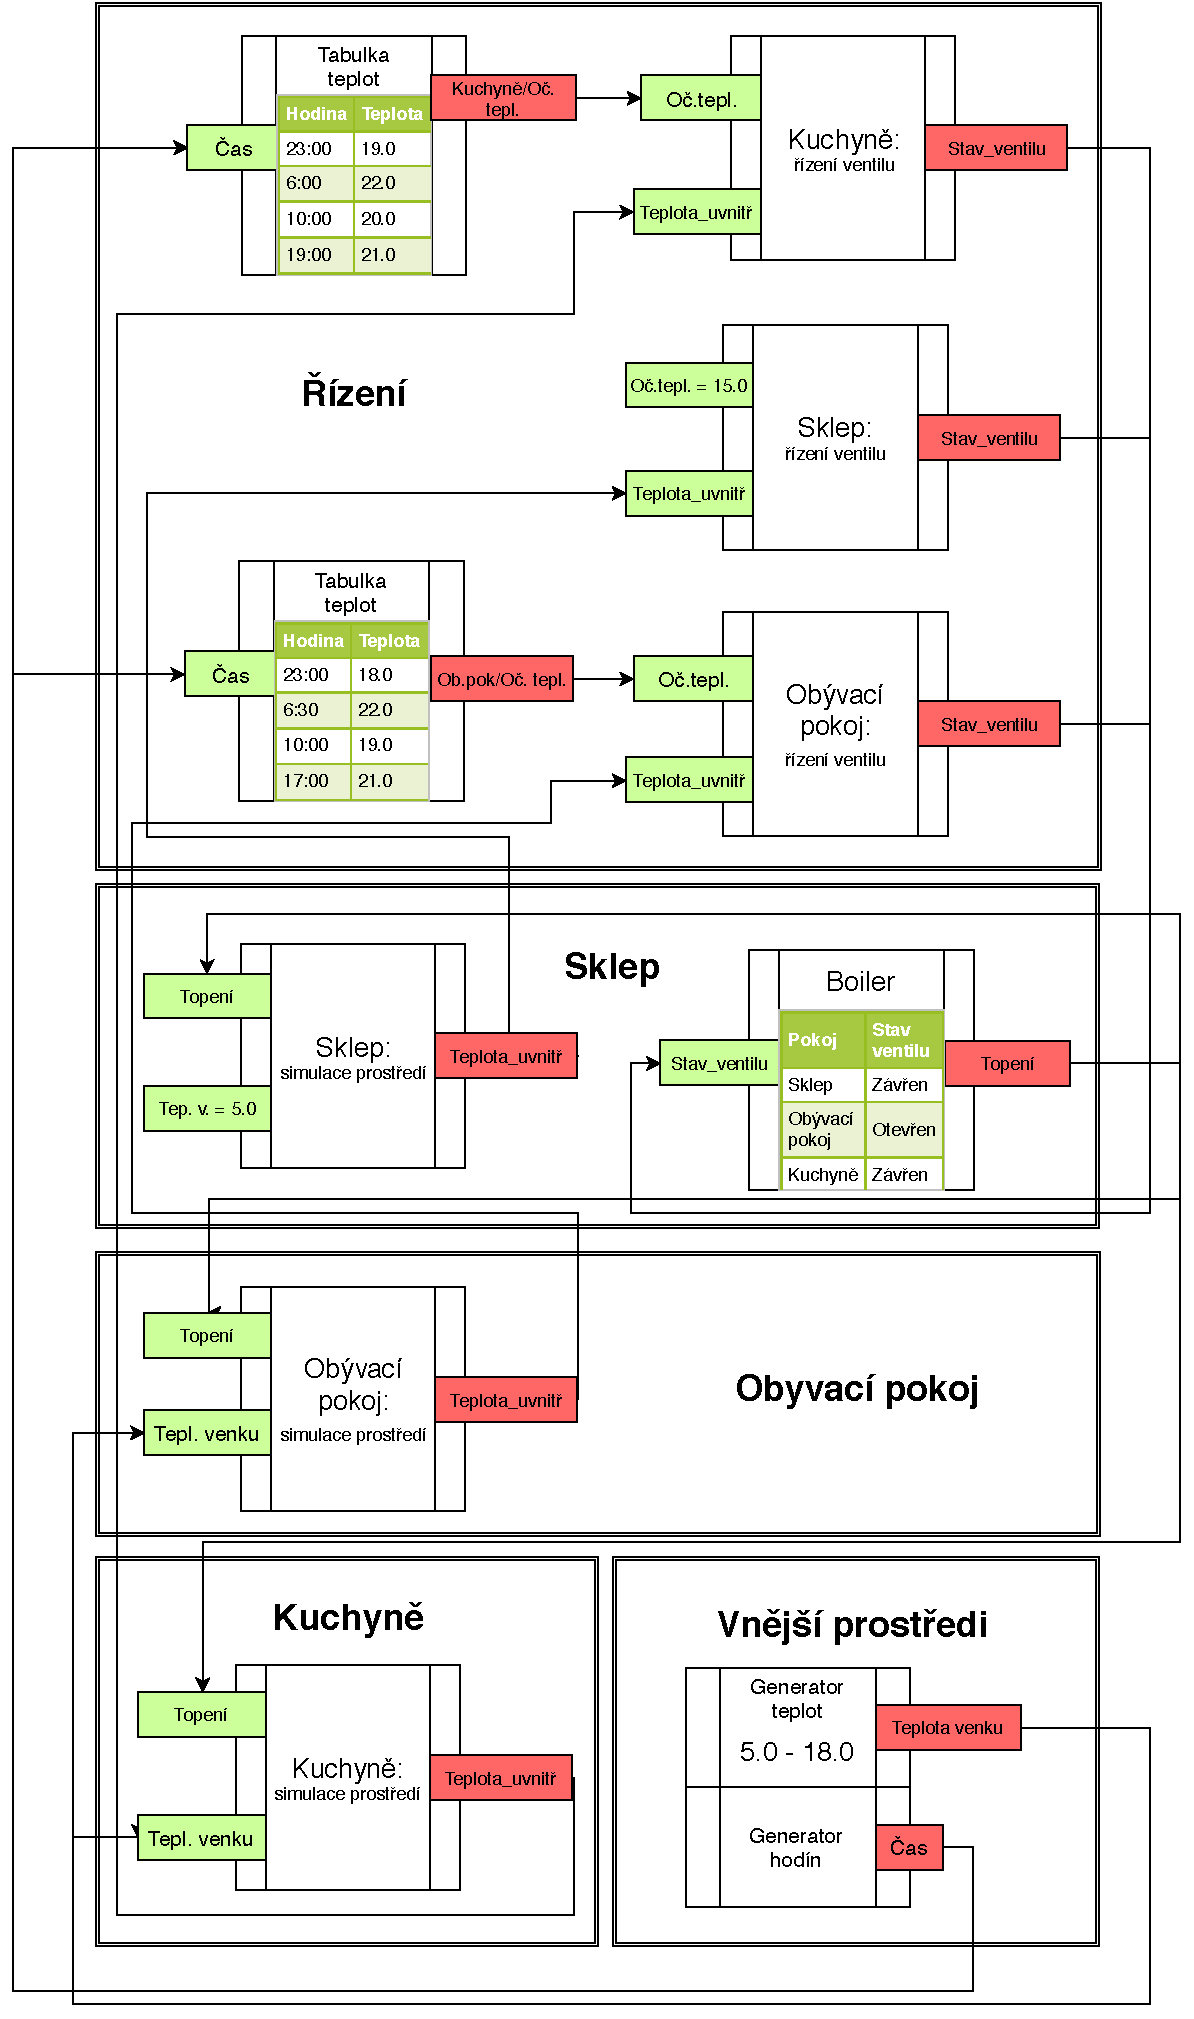
\includegraphics[width=\textwidth]{obrazky-figures/boiler-net.pdf}
  \caption{Arhitektura aplikace}
  \label{boiler-net}
\end{figure}

Aby tento navrh co nejpresneji odpovidal realite, bylo rozhodnuto namodelovat chovani teploty v pokoji.
Nejdrive musime vedet jak vykonne je topení v pokoji. Běžné hodnoty pro tři druhy pokujů mužete videt v nasledujici \hyperref[tab:TepelneZtraty]{tabulce}. Dale nas zajimaji tepelné ztraty a taky mnozstvi energii potrebne pro ohrati pokoje. Pro vypocet tohoto parametru pouzijeme nasledující vzorecek. Zakladni parametrem rozhodujicim o tepelnych kapacite pokoje je plocha vnitrniho povrchu pokoje $V$, respektive celkova plocha povrchu stopu, podlahy a sten. Pro ně je dulezte vědět koefficent ztrat tepla $K$. Zvlast se pocitaji okna a dvere, vzhledem k jejich vetshi teplovodivosti. Pak zbyva jenom zjistit rozdil současné teploty uvnitr pokoje a očekavane teploty pro tuto hodínu - $\Delta{T}$. To vsechno dosadime do vzorecku a zjistime celkové mnozstvi energii potrebne pro jeho ohrati. \cite{tep_calc}
\begin{center}
  $Q[kW/h] = \frac{V*\Delta{T}*K}{860}$
\end{center}

Pak koefficenty vypadáji nasledně:

\begin{table}[H]
	\vskip6pt
	\caption{Tabulka parametrů pokojů}
    \vskip6pt
	\centering
	\begin{tabular}{lllr}
		\toprule
		Typ pokoje & Koefficent tepelných ztrat & Objem $[m^3]$ & Očekavaný výkon topení $[W]$ \\
    \midrule
    Kuchin & 0.5 & $4*3*2.5$ & $1200$ \\
    Obývací pokoj & 0.6 & $6*4*2.5$ & $2300$ \\
    Sklep & 0.8 & $3*3*2.2$ & $300$ \\
		\bottomrule
	\end{tabular}
	\label{tab:Parametry}
\end{table}

Na vypocet tepelnych ztrat pokoje jsem pouzil \href{https://wpcalc.com/kalkulyator-teplopoter/}{tento} nastroj.
Vychazí to zhruba nasledne:

\begin{table}[H]
	\vskip6pt
	\caption{Tabulka tepelných ztrát pokojů}
    \vskip6pt
	\centering
	\begin{tabular}{llr}
		\toprule
		Typ pokoje & Ztráty $[kW/h]$ \\
		\midrule
		Kuchin & $0.7$ \\
    Pokoj & $1$ \\
    Sklep & $0.4$ \\
		\bottomrule
	\end{tabular}
	\label{tab:TepelneZtraty}
\end{table}

Cele chovani systému odpovida zákonu zachovaní energii, a tak muzeme odvodit rovnici pro vypocet potrebneho jeji mnozstvi.

\subsection{Měření teploty venku}
\label{subsec:mereni-teploty}
Modelovani chovani teploty venku je stochasticky process, ktery neni mozne spocitat presne. Proto byla navyrzena Petriho sit, vyuzivajici pravděpodobnostní přechody. Ma na vstupu rozsah teplot den - noc, a podle vybrane doby dne, za pouziti funkcii $cos$ modeluje zmenu aktualni teploty. Rozhodnuti pouziti funkce $cos$ vychazi z jednoducheho pozorovani prubehu teplot behem dne, a pereodicita zmeny teplot ji trochu \href{https://forecast.weather.gov/MapClick.php?lat=42.3758&lon=-71.1187&lg=english&FcstType=graphical}{podobá}, za predpokladu ze prubeh funkce zacina v nejteplejsi hodinu, nebo alespoň modeluje spojitý průběh teplotních změn.

Pravděpodobnostní přechody modeluji nahodne jevy jako oteplení nebo ochlazení kvůli východu sluncie nebo jiné. Vizuální reprezentací celé síťe můžete videt na obrázku \ref{thermometr-viz}.

Obrázek \ref{thermometr-viz} byl vygenerovan v průběhu práci simulatoru, díky použítí rozšíření \href{https://www.ibisc.univ-evry.fr/~fpommereau/SNAKES/API/plugins/gv.html}{\uv{gv}}. Toto rozšíření, spolu s měnšími vizualními změny jiných rozšíření, zaměřených na jednotlivé prvky sítě, dokáže spolehlívě vygenerovat obrázek Petrího sítě, podobný \ref{thermometr-viz}, v jakýkolív okámžík simulace. Táto síť je poměrně jednoduchá na pochopení, a zároveň ukazuje použítí většiny naimplementovaných rozšíření.

Pro vytvoření obrázku je specifikován jednoduchý příkaz \pyth{draw("file.png")}, a celý \hyperref[code:thermometr-draw]{postup} vypadá následně:

\begin{python}
  # Import pluginu, knihovny SNAKES, viz (*\ref{code:plugin-setup}*) (*\label{code:thermometr-draw}*)
  net_name="Thermometr"
  n=PetriNet(net_name)
  (*\ldots*) # Specifikace prechodu a mist: (*\ref{therm-gen-viz}*), (*\ref{therm-calc-viz}*) a (*\ref{prob-ev-viz}*)
  n.draw(f"{path_to_img}/{net_name}.png")
\end{python}

\begin{python}
  # Sit (*\ref{therm-gen-viz}*) (*\label{code:gen-therm-draw}*)
  f=48 # Frekvence mereni behem dne
  T=24*60*60/f # Perioda zmen teploty
  k=0 # Citac pro generator
  timeout=T
  
  # Deklarace globalnich promenych v ramci site
  n.declare(f"f={f}") (*\label{code:snakes-glob-var}*)
  
  # Vytvoreni mist
  gen=Place("Generator", [k], check=tInteger)
  gen_k=Place("Generator_k", [], check=tInteger)
  # Pridani mist do site
  n.add_place(gen)
  n.add_place(gen_k)

  # Vytvoreni prechodu
  takt=Transition("takt", timeout=timeout) (*\label{code:timed-temp-example}*)
  takt.add_input(gen, Variable("k"))
  takt.add_output(gen, Expression("(1 + k) % f"))
  takt.add_output(gen_k, Variable("k"))
  # A pridani do site
  n.add_transition(takt)
\end{python}

\begin{figure}[htb]
  \centering
  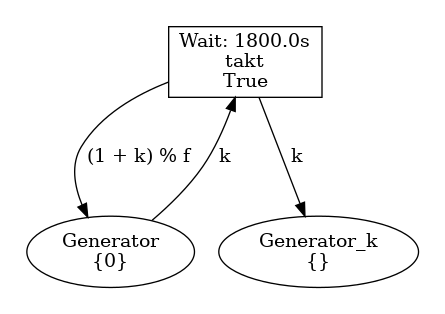
\includegraphics[width=0.4\textwidth]{obrazky-figures/therm-gen.png}
  \caption{Generator doby dne.}
  \label{therm-gen-viz}
\end{figure}

\begin{python}
  # Sit (*\ref{therm-calc-viz}*)
  # Globalni promene (*\label{code:therm-calc-draw}*)
  low, high=5, 18
  # Deklarace globalni knihovny a funkce pro vypocet teploty
  n.declare("from math import cos, pi") (*\label{code:decl-libs}*)
  n.declare("def temp_placement(Tmin, Tmax, k):" (*\label{code:decl-func}*)
  "\n\tif k == 0:"
  "\n\t\treturn float(format(Tmax, \".1f\"))"
  "\n\telse:"
  "\n\t\treturn float(format("
  "Tmin + (Tmax-Tmin)*(cos(2*pi*k/f)/2 + 1/2)," (*\label{code:lib-import-usage}*)
  "\".1f\"))")

  # Vytvoreni mist
  temp_pl=Place("Temp_placement", [(low, high)], check=tTuple)
  traw=Place("Temperature_raw", [], check=tFloat)
  n.add_place(temp_pl)
  n.add_place(traw)

  # Pridani prechodu
  tcalc=Transition("tcalc")
  tcalc.add_input(gen_k, Variable("k"))
  tcalc.add_output(traw, Expression("temp_placement(Tmin, Tmax, k)"))
  tcalc.add_input(temp_pl, Tuple((
    Variable("Tmin"), Variable("Tmax"))))
  tcalc.add_output(temp_pl, Tuple((
    Variable("Tmin"), Variable("Tmax"))))
  n.add_transition(tcalc)
\end{python}

\begin{figure}[htb]
  \centering
  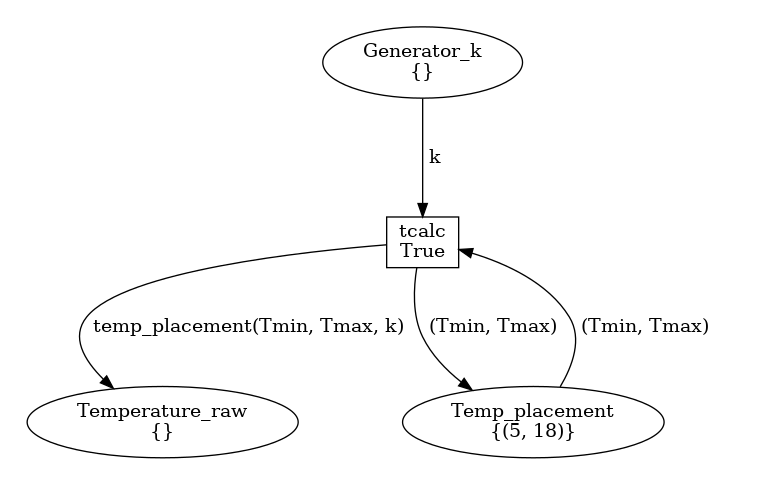
\includegraphics[width=0.6\textwidth]{obrazky-figures/calc.png}
  \caption{Výpočet teploty pro danou doubu dne.}
  \label{therm-calc-viz}
\end{figure}

\begin{python}
  # Sit (*\ref{prob-ev-viz}*)
  # Import globalnich knihoven (*\label{code:prob-ev-draw}*)
  n.declare("from random import random")

  # Pridani vystupnich mist
  meas=Place("Measurement", [0.], check=tFloat)
  n.add_place(meas)

  # Nastaveni mista jako vystupni port
  n.add_remote_output(meas, "temp_sens/Input temp")

  trainy=Transition("trainy", prob=0.2) (*\label{code:prob-temp-example}*)
  tsunny=Transition("tsunny", prob=0.2)
  texpec=Transition("texpec", prob=0.6)
  # Spojeni prechodu do skupiny
  trainy.add_neighbour_transition(texpec)(*\label{code:prob-temp-neghb-example}*)
  trainy.add_neighbour_transition(tsunny)

  # Nahodna zmena teploty vedouci k ochlazeni
  trainy.add_input(traw, Variable("Tnew"))
  trainy.add_output(meas, Expression("Tnew-random()*2"))
  n.add_transition(trainy)

  # Teplota podle ocekavani
  tsunny.add_input(traw, Variable("Tnew"))
  tsunny.add_output(meas, Expression("Tnew+random()*2"))
  n.add_transition(tsunny)

  # Zvyseni teploty na porovnani s ocekavanou
  texpec.add_input(traw, Variable("Tnew"))
  texpec.add_output(meas, Variable("Tnew"))
  n.add_transition(texpec)
\end{python}

\begin{figure}[htb]
  \centering
  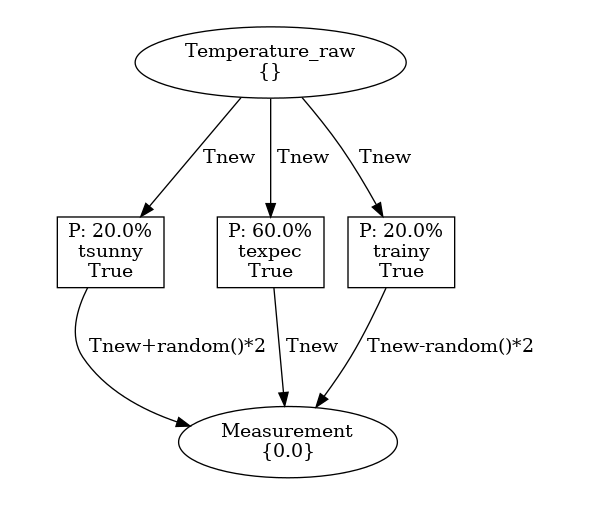
\includegraphics[width=0.6\textwidth]{obrazky-figures/measure.png}
  \caption{Modelovaní náhodných změn templot.}
  \label{prob-ev-viz}
\end{figure}

\begin{figure}[htb]
  \centering
  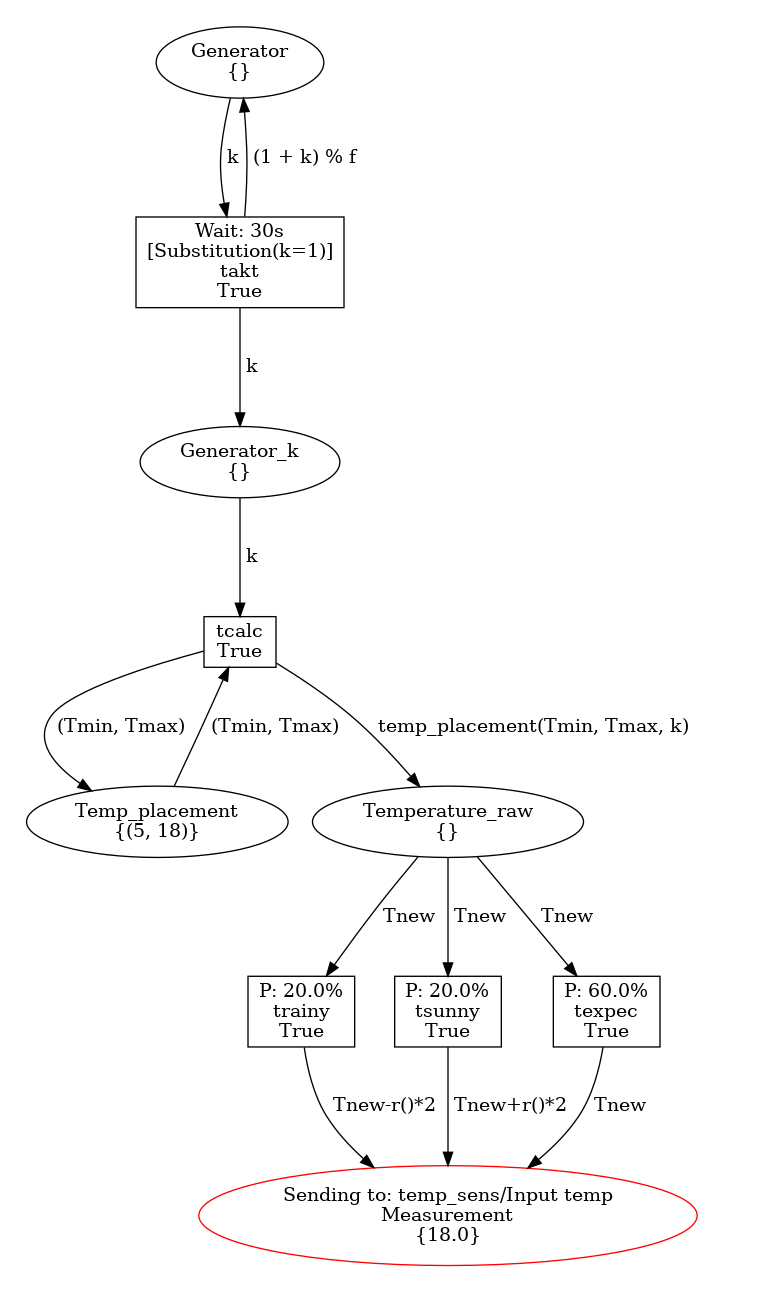
\includegraphics[width=0.7\textwidth]{obrazky-figures/thermometr.png}
  \caption{Simulace měření teploty.}
  \label{thermometr-viz}
\end{figure}

\chapter{Závěr}
\label{zaver}
